\documentclass[a4paper,norsk, 10pt]{article}
\usepackage[utf8]{inputenc}
\usepackage{verbatim}
\usepackage{listings}
\usepackage{graphicx}
\usepackage[english]{babel}
\usepackage{a4wide}
\usepackage{color}
\usepackage{amsmath}
\usepackage{float}
\usepackage{amssymb}
\usepackage[dvips]{epsfig}
\usepackage[toc,page]{appendix}
\usepackage[T1]{fontenc}
\usepackage{cite} % [2,3,4] --> [2--4]
\usepackage{shadow}
\usepackage{hyperref}
\usepackage{titling}
\usepackage{marvosym }
%\usepackage{subcaption}
\usepackage{subfig}
\usepackage{graphicx}
\usepackage[noabbrev]{cleveref}
\usepackage{cite}
\usepackage{todonotes}


\setlength{\droptitle}{-10em}   % This is your set screw

\setcounter{tocdepth}{2}

\lstset{language=c++}
\lstset{alsolanguage=[90]Fortran}
\lstset{alsolanguage=Python}
\lstset{alsolanguage=R}
\lstset{basicstyle=\small}
\lstset{backgroundcolor=\color{white}}
\lstset{frame=single}
\lstset{stringstyle=\ttfamily}
\lstset{keywordstyle=\color{red}\bfseries}
\lstset{commentstyle=\itshape\color{blue}}
\lstset{showspaces=false}
\lstset{showstringspaces=false}
\lstset{showtabs=false}
\lstset{breaklines}
\title{STK4900 Oblig1}
\author{Daniel Heinesen, daniehei}
\begin{document}
\maketitle




\section*{Exercise 1}



\subsection*{a)}
\begin{table}[ht]
\centering
\begin{tabular}{cc}
\\[-1.8ex]\hline 
\hline \\[-1.8ex]
log.no2 &    log.cars  \\ 
\hline \\[-1.8ex] 
Min.   :1.224   & Min.   :4.127  \\ 
1st Qu.:3.214   & 1st Qu.:6.176  \\ 
Median :3.848   & Median :7.425   \\ 
Mean   :3.698   & Mean   :6.973   \\ 
3rd Qu.:4.217   & 3rd Qu.:7.793   \\ 
Max.   :6.395   & Max.   :8.349     \\ 
   \hline
\end{tabular}
\caption{Summary of the main features of \textit{log.no2} and \textit{log.cars}}\label{tab:sum_no2_cars}
\end{table}



We are looking at the variables \textit{log.no2} and \textit{log.cars}, which represents the logarithm of the measured concentration of NO$_{2}$ and the logarithmic number of cars per hour. Table \ref{tab:sum_no2_cars} shows a numerical summary of \textit{log.no2} and \textit{log.cars}. Looking at \textit{log.no2} we see that the mean is close to the median, and that they both are more or less equidistant from \textit{min} and \textit{max}, and from the first and third quartiles. This indicates that the distribution is almost symmetric, with a slight skew. Looking at \textit{log.car} we see that this is no longer the case. The mean and median is more different and lie closer to $max$ and the third quartile. This means that this distribution is very skewed.




\begin{figure*}[!htbp]
\centering
\begin{tabular}{@{}ccc@{}}
\subfloat[Box plot of the distribution of \textit{log.no2}]{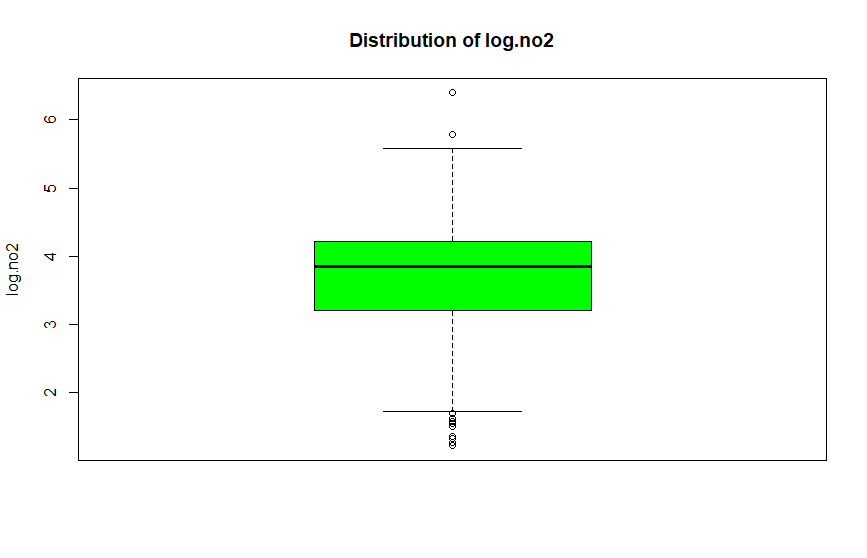
\includegraphics[width=0.5\textwidth]{box_no2.png}} & 
\subfloat[Box plot of the distribution of \textit{log.cars}]{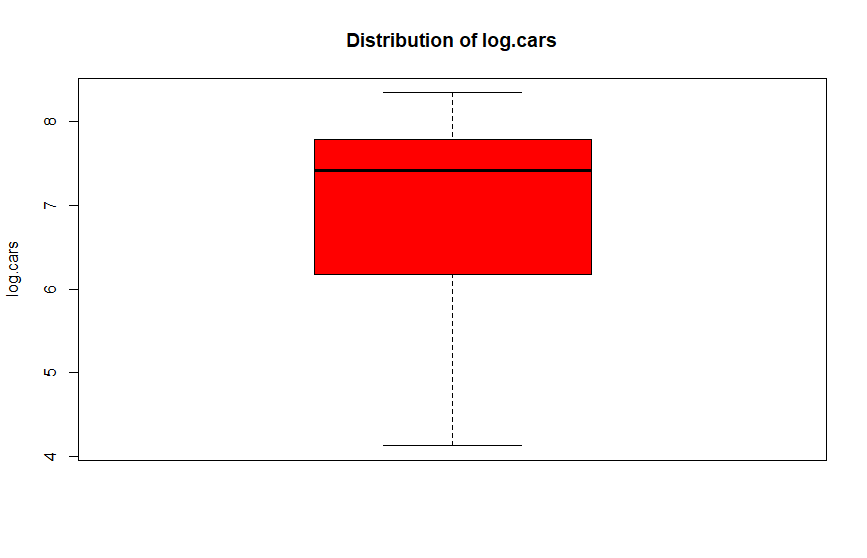
\includegraphics[width=0.5\textwidth]{box_cars.png}} &
\end{tabular}
\caption[]{Box plots showing the distributions for \textit{log.no2} and \textit{log.cars}.}
\label{fig:box_no2_cars}
\end{figure*}


Our ideas about the distribution we got from the numerical summaries, tab. \ref{tab:sum_no2_cars}, is confirmed by the box plots of the distribution found in fig. \ref{fig:box_no2_cars}. Here we can see that \textit{log.no2} is more or less symmetric, while \textit{log.cars} is heavily skewed towards higher values.

\begin{figure}[!htbp]
\centering
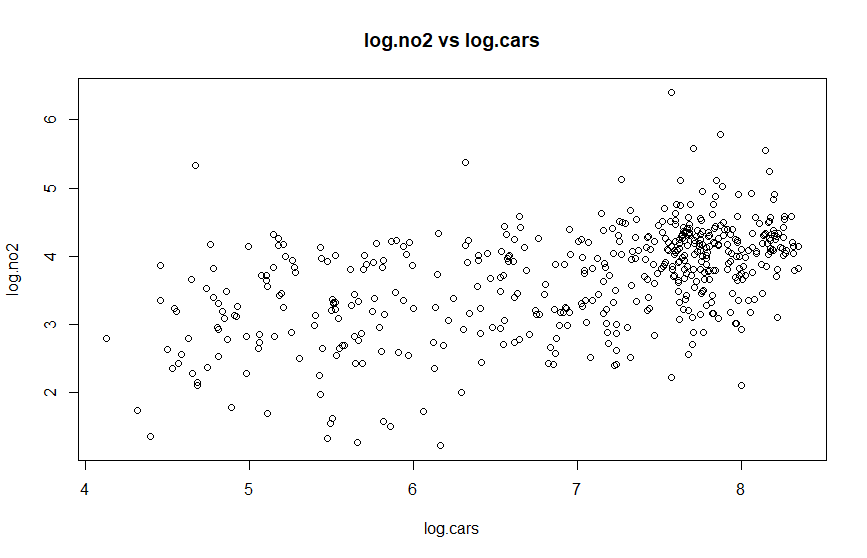
\includegraphics[scale=0.5]{no2_cars.png}
\caption{Scatter plot showing the relation between \textit{log.no2} and \textit{log.cars}.}\label{fig:no2_vs_cars}
\end{figure}

We can look at the relationship between \textit{log.no2} and \textit{log.cars}. If we look at fig. \ref{fig:no2_vs_cars} we see that there looks to be a linear dependence. We are going to try to fit a linear model to the data, but looking at the plot we see that there seems to be a higher clustering for higher values, which we expect from fig. \ref{fig:box_no2_cars}. This means that there seems to be a larger spread for lower values than for the higher, making some of the assumptions used for a linear regression false. We will look at that later.



\subsection*{b)}

We are no going to fit a linear model to our $log.no2$ and $log.cars$.


\begin{table}[!htbp]
\centering
\begin{tabular}{rrrrr}
  \hline
 & Estimate & Std. Error & t value & Pr($>$|$t$|) \\ 
  \hline
(Intercept) & 1.2331 & 0.1875 & 6.57 & 0.0000 \\ 
  log.cars & 0.3535 & 0.0266 & 13.30 & 0.0000 \\ 
   \hline
   \multicolumn{5}{l}{Residual standard error: 0.6454 on 498 degrees of freedom} \\
   \multicolumn{5}{l}{Multiple R-squared:  0.2622,	Adjusted R-squared:  0.2607} \\
   \multicolumn{5}{l}{F-statistic:   177 on 1 and 498 DF,  p-value: < 2.2e-16} \\ \hline
\end{tabular}
\caption{Summary of the linear model for $log.no2$ and $log.cars$.}\label{tab:no2_cars_fit}
\end{table}

\begin{figure}[!htbp]
\centering
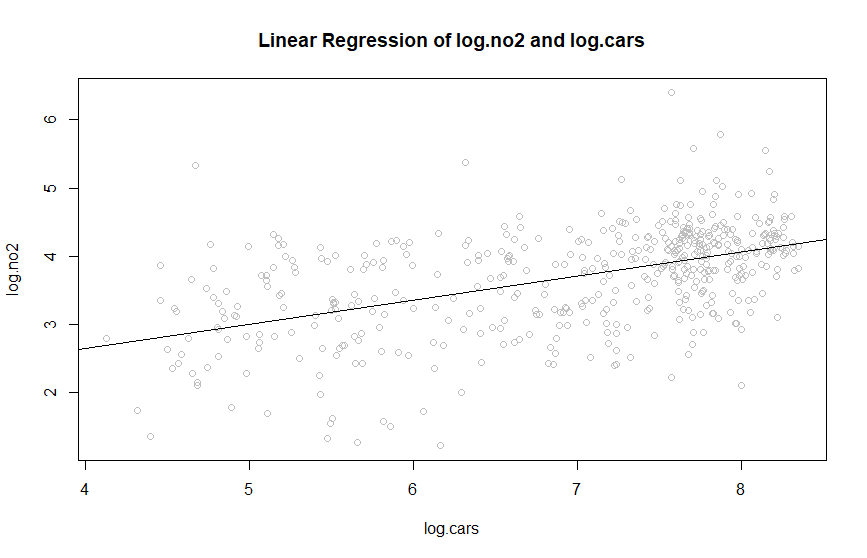
\includegraphics[scale=0.5]{no2_cars_reg.png}
\caption{The linear model superimposed on the scatter plot from fig. \ref{fig:no2_vs_cars}}\label{fig:no2_vs_cars_fit}
\end{figure}

We start by looking at fig. \ref{fig:no2_vs_cars_fit}. We can see that the line representing the linear model seems to be a good fit, but the residuals are quite large. If we look at the numerical summary in tab. \ref{tab:no2_cars_fit} we see that we get the model

\begin{equation}
log.no2 = 1.2331 + 0.3535\cdot log.cars + \epsilon.
\end{equation}

This means that given no cars on the road we expect that $log.no2 = 1.2331$, and with each additional (logarithmic) car per hour, $log.no2$ increase by $0.3535$. Looking at the p-value of $p \approx 0$ we can conclude that the linear fit is significant. But if we look at the $R^2 = 0.2622$ we see that this value is rather low. This can indicate that the data doesn't have a linear relationship -- which our p-value indicates that our data have -- or that $log.no2$ isn't described by $log.cars$ alone.


\subsection*{c)}\label{sec:c}
As mentioned above, the there seems to be a bigger spread in the data in fig. \ref{fig:no2_vs_cars_fit} for lower values than for higher ones. This is one of the things we need to look at now. 

For a linear model

\begin{equation}
y_i = \alpha + \beta_i x_i + \epsilon_i,
\end{equation}

where $\epsilon_i$ is the residuals, we need to have some assumptions.


\subsubsection*{Linearity}
For a linear regression one of the most important assumptions is that the model is linear in the predictor. We are going to check this with a  component-plus-residual plot, CPR plot. This is where we plot the partial residuals $\beta_i x_i + r_i$ against the predictor $x_i$. Since we have a model with only one predictor, this will look like our scatter plot. But R also does a smoothing of the data so that we can look at how it compares to a straight line.



\begin{figure}[!htbp]
\centering
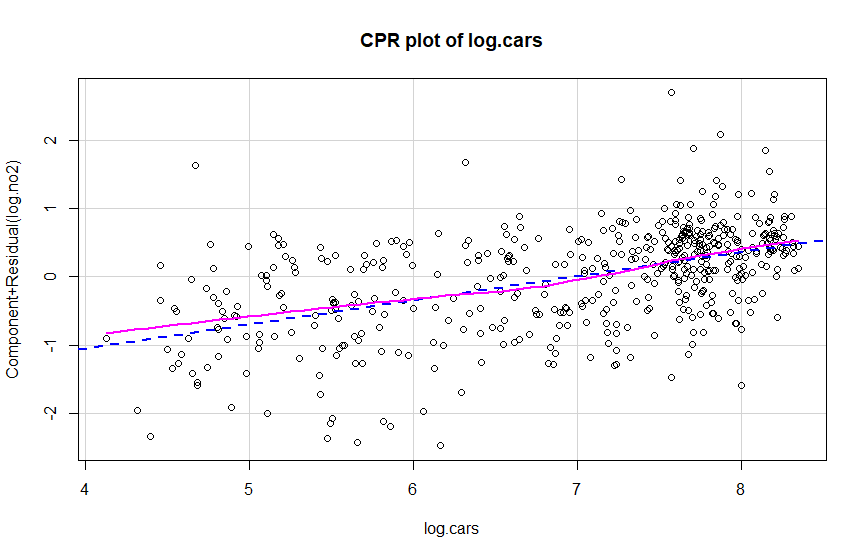
\includegraphics[scale=0.5]{cpr_cars.png}
\caption{Component-plus-residual plot of $log.cars$.}\label{fig:cpr}
\end{figure}

From fig. \ref{fig:cpr} we see that the data is somewhat linear. There is some deviation from linearity for the lower values, but  the deviation is not so great that we say that the model is non-linear.


\subsubsection*{Homoscedasticity}
For our model we want our residuals to be normally distributed with the same distribution independent of the value of $log.cars$. To check this we are going to plot the square root of the absolute value of the standardized residuals against the fitted values. We expect that the residuals there are random around a mean for all the fitted values, meaning that we can fit a straight, horizontal line  to the data. 
	
\begin{figure}[!htbp]
\centering
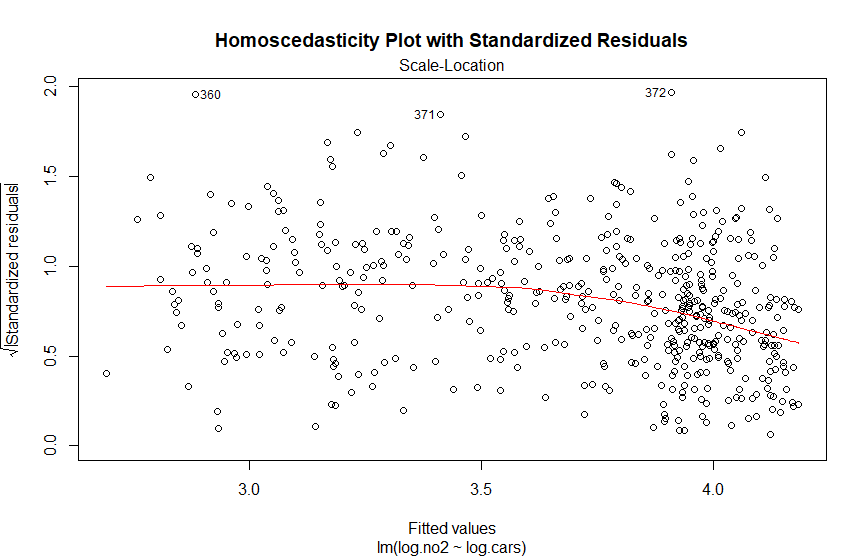
\includegraphics[scale=0.5]{stand_res.png}
\caption{Figure showing $\sqrt{|\text{Standardized Residuals}|}$ against the fitted values.}\label{fig:stand_res}
\end{figure}

Looking at fig. \ref{fig:stand_res} we would expect to see a straight line, meaning that residuals have same distribution, but we see that for the lower fitted values, $\sqrt{|\text{Standardized Residuals}|}$ is higher than for higher values. This indicates that the residuals as smaller for larger values of $log.cars$. This seems to verify what we expected from the start: That there was a larger spread for the smaller values of $log.cars$ than for the larger.


\subsubsection*{Normality} 
The last assumption we have is that the residuals are normal. 

\begin{figure}[!htbp]
\centering
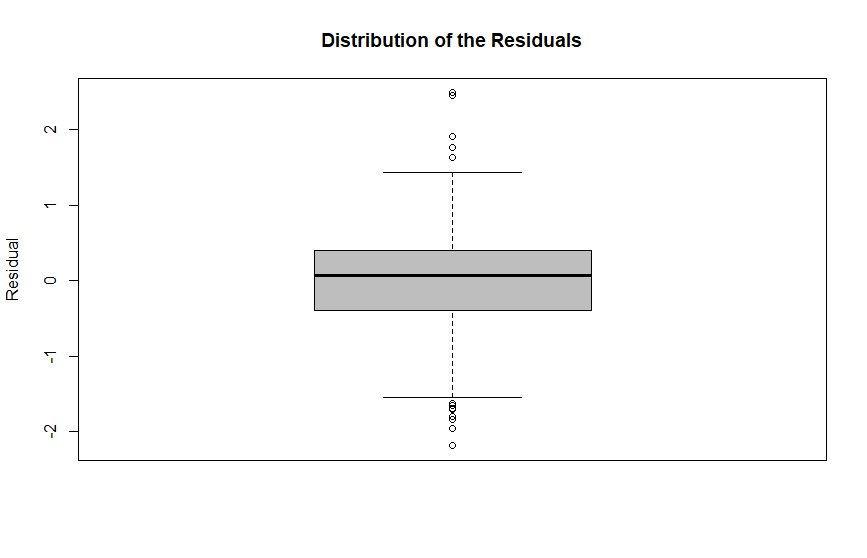
\includegraphics[scale=0.5]{res_box.png}
\caption{Figure a box plot of the residuals.}\label{fig:res_box}
\end{figure}

\begin{figure}[!htbp]
\centering
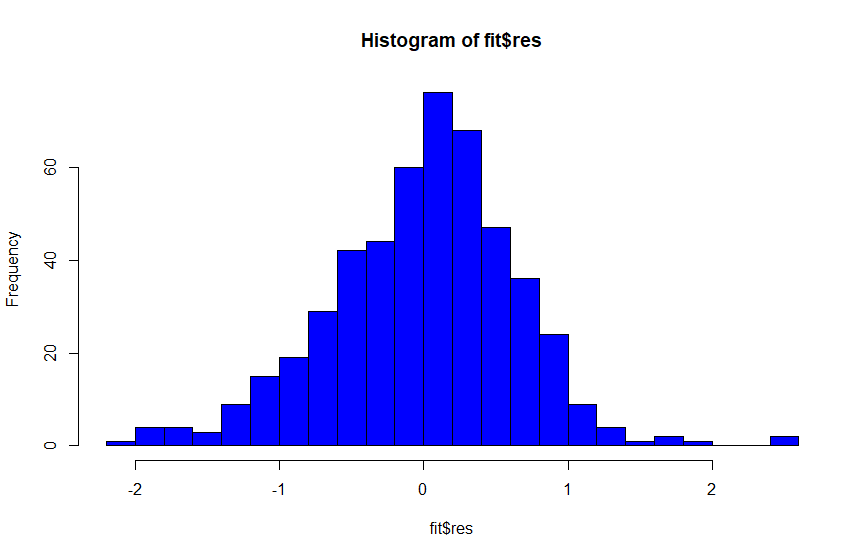
\includegraphics[scale=0.5]{res_hist.png}
\caption{Figure the histogram of the residuals.}\label{fig:res_hist}
\end{figure}

\begin{figure}[!htbp]
\centering
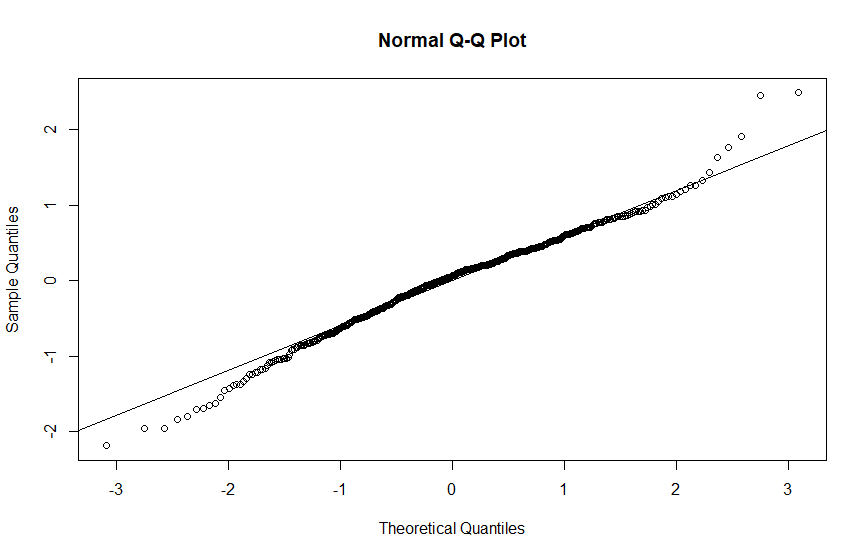
\includegraphics[scale=0.5]{res_qq.png}
\caption{Figure a QQ-plot of the residuals.}\label{fig:res_qq}
\end{figure}


Looking at fig. \ref{fig:res_box} we see that the distribution looks more or less normal, but the median is somewhat of center, which indicates skewness. Fig. \ref{fig:res_hist} shows that this is the case. The distribution is far from normal, and seems to be skew towards the negative values. From both these figures we can see that neither the median nor the mean is $0$, which is something we would like it to be.

The last nail in the coffin is fig. \ref{fig:res_qq}. If the residuals were normally distributed, we would expect a the points to follow the straight line. The S-shape indicates a light tail, and the bend we see in the middle indicates a left skew -- which corresponds well with our other plots --. This means that our assumptions that the residuals are normally distributed is false.


So we have seen that while our model is close to linear, the residuals are neither homoscedastic nor normal. So to use a linear model for our data can be difficult to justify.



\subsection*{d)}

Our data consists of more possible predictor variables than just $log.cars$. We have three more variables we can use in a multiple regression. To see which if these variables we are going to use, we are going to do a \textit{forward selection} of the variables and their logarithm: We start by making a linear model with each predictor variable (and their logarithm), using \textbf{Cross Validated} $R^2$ we will find the best model. We then goes through the remaining variables, adding that to the best predictor and see which variable improves the fit. This is done recursively until there is no improvement in the cross validated $R^2$. We then have our best model. 

Due to my lack in familiarity with R, this was done in the stupid way of checking each combination one by one. 


\begin{figure}[!htbp]
\centering
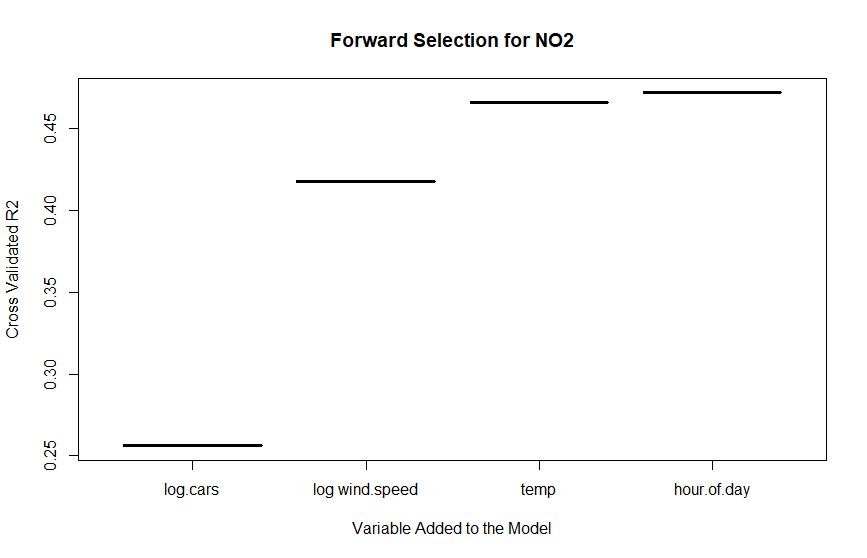
\includegraphics[scale=0.5]{r2_forward.png}
\caption{Figure of the increase in the cross validated $R^2$ as variable are added. The x-axis shows which predictor variable is added to the model.}\label{fig:r2}
\end{figure}


We see from fig. \ref{fig:r2} that as we add more predictor variables the model becomes better and better. We also notice that to get the best model we also had to take the logarithm of $wind.speed$. The model we are left with then is found in tab. \ref{tab:r2},and can be written as

\begin{equation}\label{eq:full}
log.no2 = 1.07 + 0.46\cdot log.cars - 0.42\cdot \log(wind.speed) - 0.03\cdot temp - 0.01 \cdot hour.of.day + \epsilon
\end{equation}

\begin{table}[ht]
\centering
\begin{tabular}{rrrrr}
  \hline
 & Estimate & Std. Error & t value & Pr($>$|$t$|) \\ 
  \hline
(Intercept) & 1.0709 & 0.1710 & 6.26 & 0.0000 \\ 
  log.cars & 0.4572 & 0.0279 & 16.37 & 0.0000 \\ 
  log(wind.speed) & -0.4194 & 0.0364 & -11.53 & 0.0000 \\ 
  temp & -0.0267 & 0.0038 & -6.96 & 0.0000 \\ 
  hour.of.day & -0.0123 & 0.0044 & -2.81 & 0.0051 \\ 
   \hline
      \multicolumn{5}{l}{Residual standard error: 0.542 on 495 degrees of freedom} \\
   \multicolumn{5}{l}{Multiple R-squared:  0.483,	Adjusted R-squared:  0.479 } \\
   \multicolumn{5}{l}{F-statistic:  116 on 4 and 495 DF,  p-value: <2e-16} \\ \hline
\end{tabular}
\caption{Table showing the final model for our multiple regression. This is the model which gives the best cross validation $R^2$.}\label{tab:r2}
\end{table}


\subsection*{e)}

\subsubsection*{Checking our Assumptions}

We will now check if our model assumptions are correct. We will do the exact same analysis as in exercise 1c. We will do it a bit quicker now since we have done it once before.


\begin{figure*}[!htbp]
\centering
\begin{tabular}{@{}ccc@{}}
\subfloat[CPR plot for the full model]{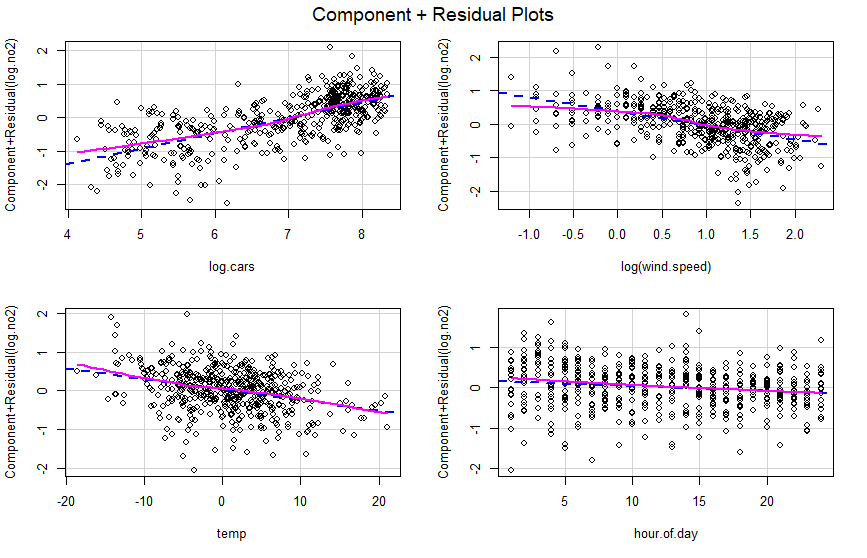
\includegraphics[width=0.5\textwidth]{cpr_full.png}} & 
\subfloat[Standard Residual plot for the full model]{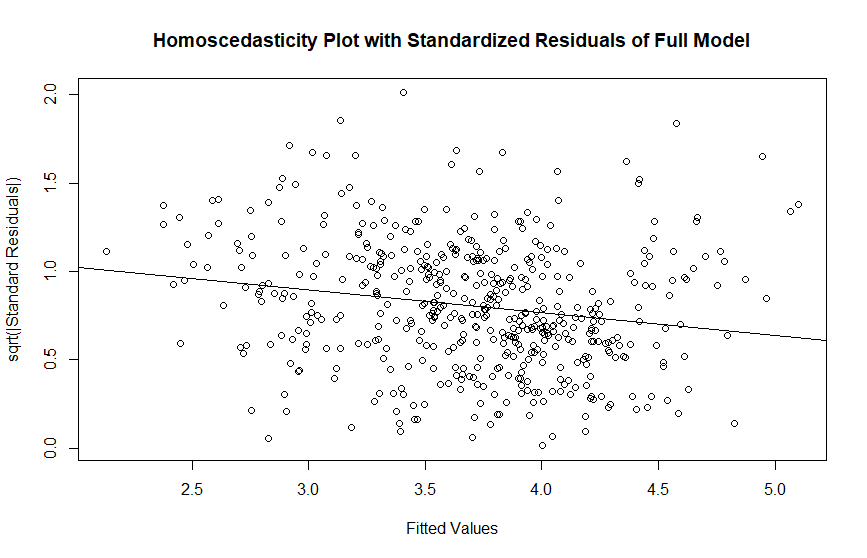
\includegraphics[width=0.5\textwidth]{stand_full.png}} &
\end{tabular}
\caption[]{Plots judging the linearity and homoscedasticity of the residuals of the full model.}
\label{fig:cpr_and_stand}
\end{figure*}

\begin{figure*}[!htbp]
\centering
\begin{tabular}{@{}cccc@{}}
\subfloat[Box plot for the residuals for the full model]{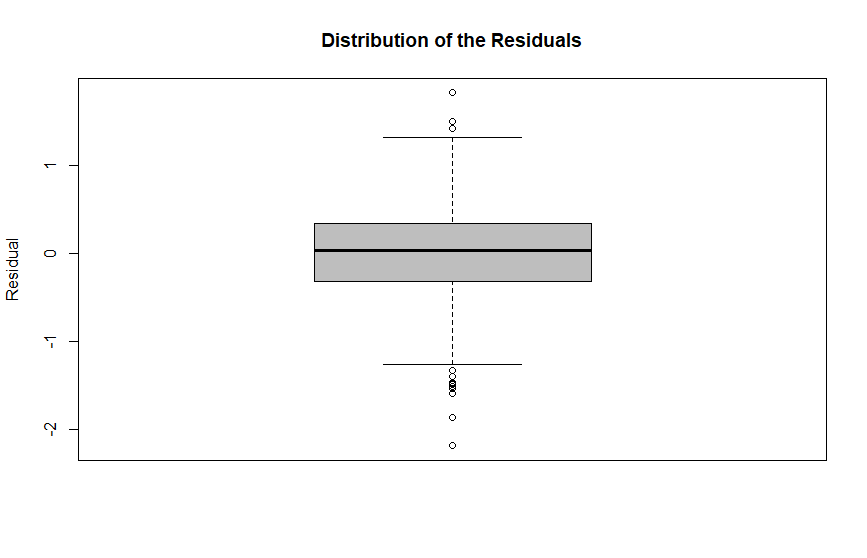
\includegraphics[width=0.33\textwidth]{box_full.png}} & 
\subfloat[Histogram for the residuals for the full model]{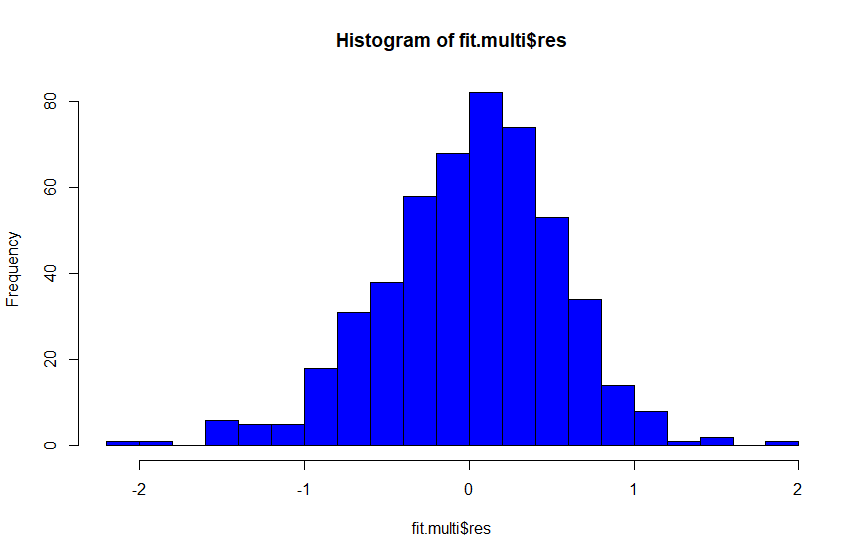
\includegraphics[width=0.33\textwidth]{hist_full.png}} &
\subfloat[QQ plot for the residuals for the full model]{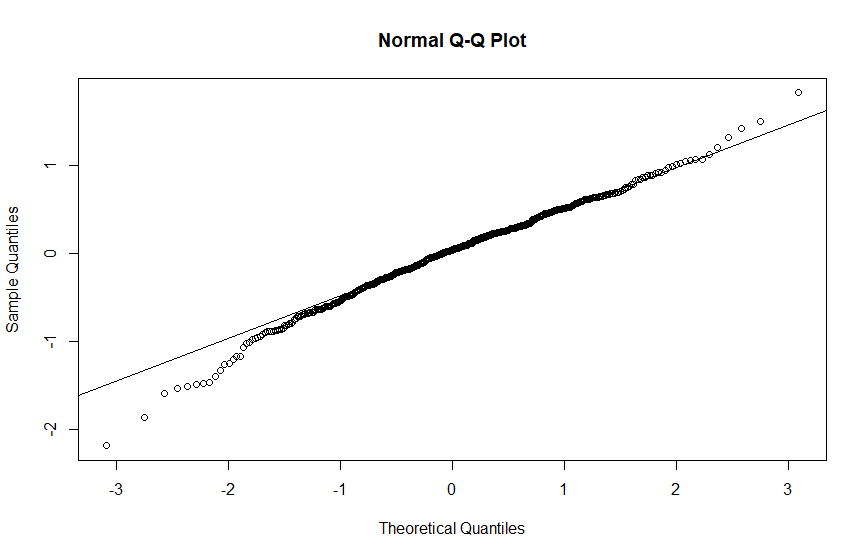
\includegraphics[width=0.33\textwidth]{qq_full.png}} &
\end{tabular}
\caption[]{Plots judging the normality of the residuals of the full model.}
\label{fig:normal_full}
\end{figure*}



Fig. \ref{fig:cpr_and_stand}a shows that $temp$ and $hour.of.day$ seems to be more or less linear, while $log wind.speed$ has some small deviations from linearity. It is close enough that we can say that our model is linear.

Fig. \ref{fig:cpr_and_stand}b shows that we still have the problem with varying residuals, which is problematic for our assumption of homoscedasticity.

From the plots in fig. \ref{fig:normal_full} we see that the residuals are a bit non-normal still. If we only look at the values close to the mean we see that the QQ-plot indicates these to be normal. It is the outliers -- as judged by the box plot -- that seems to be breaking normality. Excluding these, we can say that the residuals are normally distributed for the full model. 


\subsubsection*{Interpreting our Model}
If we look at \eqref{eq:full} and tab. \ref{tab:r2} we can see that the base value of $log.no2$ is $1.07$, and for each (logarithmic) car per hour this value is increased with $0.46$, and with each extra (logarithm) $m/s$ of wind speed it is decreased with $0.42$. With $1^{\circ}$C increase in temperature the $log.no2$ is decreased with $0.03$. And lastly with one hour later in the day, it is decreased with $0.01$.

We see that we get a $R^2$ value of $0.483$, which is significantly higher than with our model in tab. \ref{tab:sum_no2_cars}. It is still not close to $1$, so there is some other factors that helps determine $log.no2$.

So all in all, we have a good model, which fulfill most of our assumptions of a linear model.





\section*{Exercise 2}

\subsection*{a)}

The data we are looking at is the systolic blood pressure for $36$ people divided into three groups determined by their age. These groups are $30-45$ years, $46-59$ years and $60-75$ years. 

\begin{table}[!htbp] \centering 

\begin{tabular}{@{\extracolsep{5pt}}lccccccc}  
\\[-1.8ex]\hline 
\hline \\[-1.8ex] 
Age Group & \multicolumn{1}{c}{N} & \multicolumn{1}{c}{Mean} & \multicolumn{1}{c}{St. Dev.} & \multicolumn{1}{c}{Min} & \multicolumn{1}{c}{Pctl(25)} & \multicolumn{1}{c}{Pctl(75)} & \multicolumn{1}{c}{Max} \\ 
\hline \\[-1.8ex] 
All & 36 & 138.806 & 25.749 & 104 & 117.5 & 156.2 & 214 \\ 
$30-45$ years & 12 & 122.167 & 15.338 & 104 & 112 & 129 & 160 \\
$46-59$ years & 12 & 139.083 & 22.625 & 108 & 121.5 & 157.8 & 174 \\ 
$60-75$ years & 12 & 155.167 & 27.719 & 110 & 138 & 164 & 214 \\
\hline \\[-1.8ex] 
\end{tabular} 
\caption{A table showing different measures for the distribution of the systolic blood pressure for the three age groups, and the entire group as a whole. The increase in all the measures for the higher age groups seems to indicate a correlation between age and blood pressure.}   \label{tab:blood_summary} 

\end{table} 


If we look at table \ref{tab:blood_summary} we see the numerical summary of the blood pressure of the three age groups, and the group as a whole. From the mean column, we see that mean blood pressure seems to increase with increasing age group. This is also the case for all the other measures see in the table. This seems to indicate that there is some relationship between systolic blood pressure and age.


\begin{figure}[!htbp]
\centering
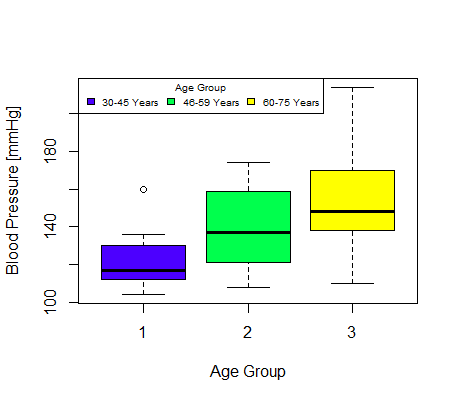
\includegraphics[scale=0.8]{blood_box.png}
\caption{Boxplots showing the distribution of the blood pressure of the three age groups.}\label{fig:blood_box}
\end{figure}


From fig. \ref{fig:blood_box} we see that there is a clear increase in blood pressure with age. Both the median, max and min increases with age. This is exactly what we saw in tab. \ref{tab:blood_summary} -- a difference is that in the table the mean was given, while in the box plot the median is given --. What we can see clearer from the plot is that the distributions also become wider as age increase. The interquartile width of the middle age group is quite wide, and overlaps with the other groups. This can make this group a bit more difficult to get a significant result from.

All in all, both the numerical summary, tab. \ref{tab:blood_summary}, and the box plot, fig. \ref{fig:blood_box}, seems to show the same: There seems to be variation in systolic blood pressure across the different age groups.

\subsection*{b)}

We now want to look close at whether blood pressure varies between the different age groups. Above we used qualitative reasoning to to argue that this is the case. Now we want a quantified measure of this. To do this we will use a one-way ANOVA. 

For the ANOVA we have the following hypotheses:
\begin{itemize}
  \item $H_0: \mu_1 = \mu_2 = \mu_2$
  \item $H_a:  \mu_1 \neq \mu_2 \neq \mu_2$
\end{itemize}

In words: We have a null hypothesis that the mean blood pressure of all the groups are the same, and an alternative hypothesis that this is not that case. For the ANOVA to be valid, we need to assume that: 

\begin{itemize}
  \item The observations are independent of one another
  \item The observations in one group are a random sample with a normal distribution $N(\mu_k,\sigma^2)$
\end{itemize} 



% latex table generated in R 3.5.2 by xtable 1.8-3 package
% Thu Mar 07 14:02:58 2019
\begin{table}[!htbp]
\centering
\begin{tabular}{lrrrrr}
  \hline
 & Df & Sum Sq & Mean Sq & F value & Pr($>$F) \\ 
  \hline
Age Group & 2 & 6535.39 & 3267.69 & 6.47 & 0.0043 \\ 
  Residuals & 33 & 16670.25 & 505.16 &  &  \\ 
   \hline
\end{tabular}
\caption{A table showing the result of an ANOVA test on the blood pressure dataset. We see that we have a high F-value, leading to a small, significant p-value.}\label{tab:blood_anova}

\end{table}


From tab. \ref{tab:blood_anova} we see that we get a small p-value of $p=0.0043$. This is below the $p=0.05$ mark which is standard to use as the limit of significance. This means that we can throw out that null hypothesis, and conclude that blood pressure indeed varies across the age groups \footnote{It is normally bad practice to interpret the p-value in an article, but since this is an oblig, it is done here.}


\subsection*{c)}

We are now going to try to use a categorical regression on the data set. We are going to use treatment-contrast with group 1, the youngest, as the reference group. This means that our model will look like

\begin{equation}
y_i = \mu_1 + (\mu_2-\mu_1)\cdot x_{1,i} + (\mu_2-\mu_1)\cdot x_{2,i} + \epsilon_i,
\end{equation}

where $\epsilon_i$ is a normally distributed error term, $\mu_j$ is the mean of the different age groups, and

\begin{equation}
x_{j-1,i} = 
\begin{cases}
1 \text{	for $i$ in group $j$} \\
0 \text{	else}
\end{cases}.
\end{equation}
This means that if patient is in group 2, then $x_{1,i} = 1$ and $x_{2,i} = 0$, and vis versa if the patient is in group 3. If the patient is in group 1, both will be $0$.

% latex table generated in R 3.5.2 by xtable 1.8-3 package
% Thu Mar 07 15:06:19 2019
\begin{table}[!htbp]
\centering
\begin{tabular}{rrrrr}
  \hline
 & Estimate & Std. Error & t value & Pr($>$ $|$t$|$) \\ 
  \hline
(Intercept) & 122.1667 & 6.4882 & 18.83 & 0.0000 \\ 
  Age Group 2 & 16.9167 & 9.1757 & 1.84 & 0.0742 \\ 
  Age Group 3 & 33.0000 & 9.1757 & 3.60 & 0.0010 \\ 
  \hline
   \multicolumn{5}{l}{Residual standard error: 22.48 on 33 degrees of freedom} \\
	\multicolumn{5}{l}{Multiple R-squared:  0.2816,	Adjusted R-squared:  0.2381} \\
	\multicolumn{5}{l}{F-statistic: 6.469 on 2 and 33 DF,  p-value: 0.004263} \\
   \hline
\end{tabular}
\caption{The summary of the categorical regression of the blood pressure with respect to the age groups.}\label{tab:blood_reg}
\end{table}

In tab. \ref{tab:blood_reg} we see the summary of the regression model with the age groups as a categorical predictor variable. The intercept in the table is the mean of the youngest age group $\mu_1 = 122.167$ --  our reference group --. The slopes of the two variables can be interpreted as how much the mean of blood pressure increases if you are in that age group, compared to the reference group. E.g. if you are in age group 2, we will expect your blood pressure to be $33.0$ mmHg higher than the mean of the youngest group, i.e. it is expected to be $155.167$ mmHg.

We can look at the p-values of tab. \ref{tab:blood_reg} we see that the p-value for age group 3 is $p=0.001$. This means that the increase of $33$ mmHg is significant. But for group 2 the p-value is just $0.0742$, which means that this increase is not significant, meaning that we can't say that this is due to age and not due statistical error. This might have to do with what we see in the box plots \ref{fig:blood_box}, where the distribution of the second age group is very wide. The reason might also be due to a non linear dependence on age.

We also see that we have a low $R^2 = 0.2816$, which means that the blood pressure is not fully described by the age groups.

But all in all we see that the we have a good regression model for group 1 and 3, with the change in group 2 not being significant. So there is some significant variation between the age groups, as we saw with the ANOVA. But while the ANOVA only showed that there was a variation across the different age groups, the linear regression show that we have an increase in the blood pressure for the higher age groups.

\section*{Remark}
I have collaborated with \textit{Simon Millerjord}. This is especially true for the R code, and plots!


\newpage
\section*{Appendix}
\subsection*{R Code for Problem 1}

\lstinputlisting{../problem1.R}

\newpage

\subsection*{R Code for Problem 2}

\lstinputlisting{../problem2.R}


\end{document}

